% This is the Reed College LaTeX thesis template. Most of the work
% for the document class was done by Sam Noble (SN), as well as this
% template. Later comments etc. by Ben Salzberg (BTS). Additional
% restructuring and APA support by Jess Youngberg (JY).
% Your comments and suggestions are more than welcome; please email
% them to cus@reed.edu
%
% See https://www.reed.edu/cis/help/LaTeX/index.html for help. There are a
% great bunch of help pages there, with notes on
% getting started, bibtex, etc. Go there and read it if you're not
% already familiar with LaTeX.
%
% Any line that starts with a percent symbol is a comment.
% They won't show up in the document, and are useful for notes
% to yourself and explaining commands.
% Commenting also removes a line from the document;
% very handy for troubleshooting problems. -BTS


%%%%%%%%%%%%%%
%% Preamble %%
%%%%%%%%%%%%%%
% \documentclass{<something>} must begin each LaTeX document
\documentclass{ufdissertation}[overrideChapters] %UF's 2019 Template --ANF
%Packages are extensions to the basic LaTeX functions. Whatever you want to
%typeset, there is probably a package out there for it. Chemistry (chemtex),
%screenplays, you name it. Check out CTAN to see: https://www.ctan.org/ Also,
%Rmarkdown can read LaTex commands in Rmd files, so long as the output is a pdf,
%because pdfs are rendered by Rmarkdown via LaTex
%%
\usepackage{siunitx}
\usepackage{textgreek}
% \usepackage[section]{placeins}
\usepackage{pdfpages}
\usepackage{calc}
\usepackage{rotating}

% Syntax highlighting #22

% So, this code uses your CSL file to decide how to format your citations
% You may need to edit your CSL if the editorial office doesn't like it
% From {rticles}
\newlength{\csllabelwidth}
\setlength{\csllabelwidth}{3em}
\newlength{\cslhangindent}
\setlength{\cslhangindent}{1.5em}
% for Pandoc 2.8 to 2.10.1
\newenvironment{cslreferences}%
  {}%
  {\par}
% For Pandoc 2.11+
% As noted by @mirh [2] is needed instead of [3] for 2.12
\newenvironment{CSLReferences}[2] % #1 hanging-ident, #2 entry spacing
 {% don't indent paragraphs
  \setlength{\parindent}{0pt}
  % turn on hanging indent if param 1 is 1
  \ifodd #1 \everypar{\setlength{\hangindent}{\cslhangindent}}\ignorespaces\fi
  % set entry spacing
  \ifnum #2 > 0
  \setlength{\parskip}{#2\baselineskip}
  \fi
 }%
 {}
\usepackage{calc} % for calculating minipage widths
\newcommand{\CSLBlock}[1]{#1\hfill\break}
\newcommand{\CSLLeftMargin}[1]{\parbox[t]{\csllabelwidth}{#1}}
\newcommand{\CSLRightInline}[1]{\parbox[t]{\linewidth - \csllabelwidth}{#1}}
\newcommand{\CSLIndent}[1]{\hspace{\cslhangindent}#1}

\providecommand{\tightlist}{%
  \setlength{\itemsep}{0pt}\setlength{\parskip}{0pt}}
% % Added by CII (Thanks, Hadley!)
% % Use ref for internal links
\renewcommand{\hyperref}[2][???]{\autoref{#1}}
\def\chapterautorefname{Chapter}
\def\sectionautorefname{Section}
\def\subsectionautorefname{Subsection}
% End of CII addition
\begin{document}
\docBodyfalse
%%%%%%%%%%%%%%%%%%%%%%%%%%%%%%%%%
% TITLE PAGE                    %
%%%%%%%%%%%%%%%%%%%%%%%%%%%%%%%%%
    \begin{center}
        \thispagestyle{empty}%
        \vspace*{-0.4in}\realSingleSpace{DETECTION OF TWO MITE-PLANT-VIRUS PATHOSYSTEMS IN FLORIDA, INCLUDING CHEMICAL ECOLOGY OF \emph{Amblyseius swirskii} and INDUCTION OF SYSTEMIC ACQUIRED RESISTANCE ON ROSES}%
        \vfill%
        By \\*[\baselineskip]%
        \MakeUppercase{Austin N Fife}%
        \vfill%
        A \MakeUppercase{Dissertation} PRESENTED TO THE GRADUATE SCHOOL \\%
        OF THE UNIVERSITY OF FLORIDA IN PARTIAL FULFILLMENT \\%
        OF THE REQUIREMENTS FOR THE DEGREE OF \\%
        \MakeUppercase{Doctor of Philosophy} \\*[\baselineskip]%
        UNIVERSITY OF FLORIDA \\*[\baselineskip]%
        {2021}%
    \end{center}
    \newpage

%%%%%%%%%%%%%%%%%%%%%%%%%%%%%%%%%
% COPYRIGHT PAGE                %
%%%%%%%%%%%%%%%%%%%%%%%%%%%%%%%%%
    \newpage
      \vspace*{\fill}
        \begin{center}
            \textcopyright{} {2021} {Austin N Fife}
        \end{center}
      \vspace*{\fill}
    \newpage

\setcounter{secnumdepth}{-1}     % We don't want chapter numbers until later,
                                 % So let's kill off the table of contents depth detector until we want to start counting.
                                 

%%%%%%%%%%%%%%%%%%%%%%%%%%%%%%%%%
% DEDICATION                    %
%%%%%%%%%%%%%%%%%%%%%%%%%%%%%%%%%

    \vspace*{\fill}               % We want the dedication to be centered,
                                  % So we use \vspace*{\fill} above and below.
\begin{center}                    % We also want to center the dedication horizontally.
  \realSingleSpace
  {For Liz, Violet, Juniper and Fifes to come}
\end{center}
\vspace*{\fill}                   % Note that the * in \vspace* is necessary,
                                  % as otherwise latex will ignore it here


%%%%%%%%%%%%%%%%%%%%%%%%%%%%%%%%%
% ACKNOWLEDGMENTS               %
%%%%%%%%%%%%%%%%%%%%%%%%%%%%%%%%%

{\hypertarget{acknowledgments}{%
\chapter{ACKNOWLEDGMENTS}\label{acknowledgments}}

I would like to give special thanks for the Tallahassee Museum and their patience, cooperation, and support with collecting plant samples. I am thankful for the USDA-APHIS PPQ Beltsville laboratory for their support in the identification and confirmation OFV isolates, as well as \emph{Brevipalpus} mite identification at the USDA-ARS. I also want to recognize Drs. Sam Bolton, FDACS and Aline Tassi, Univ. of Sao Paulo, Brazil for checking the mites we have sent for species validation. I appreciate Dr.~Marc S. Frank's helpful identification of the Liriopogons collected. I am especially beholden to the late Dr.~Gary Bauchan for his brilliant Cryo-SEM images, and his contributions to the field of acarology. He will be greatly missed. This research was partly funded by the USDA National Institute of Food and Agriculture, Hatch project FLA-NFC-005607 and USDA-AFRI-CPPM 2017-70006-27268. Funds were also contributed by The Florida Nursery, Growers and Landscape Association's (FNGLA) Endowed Research Funds. Mention of trade names or commercial products in this publication is solely for the purpose of providing specific information and does not imply recommendation or endorsement by the USDA; USDA is an equal opportunity provider and employer. I am thankful for the time, patience, and dedication of my committee members Drs. Gary Knox and Daniel Carrillo. I am also incredibly grateful to my Co-PIs, Dr.~Mathews Paret and Dr.~Xavier Martini, who have helped to lead, guide, inspire, and redirect me on the path to becoming a young researcher. I am obliged to my goodly parents for teaching me about the importance of learning, and for the heritage and language of my maternal grandmother, which has blessed my life so much. \emph{Los abuelos nunca mueren, sólo se vuelven invisibles.} Most of all, I am eternally indebted to my spouse, Liz, as well as my daughters Violet and Juniper for their endurance and support during these most harrowing years of my life. Thank you.}              % Inputs the text found in the 00-acknowledgments.Rmd file


%%%%%%%%%%%%%%%%%%%%%%%%%%%%%%%%%
% TABLE OF CONTENTS             %
%%%%%%%%%%%%%%%%%%%%%%%%%%%%%%%%%

 \realSingleSpace
  \tableofcontents % Table of Contents comes fourth.


%%%%%%%%%%%%%%%%%%%%%%%%%%%%%%%%%
% LIST OF TABLES                %
%%%%%%%%%%%%%%%%%%%%%%%%%%%%%%%%%

  \listoftables  % List of tables comes next, if you have one.
  \addcontentsline{toc}{chapter}{LIST OF TABLES}


%%%%%%%%%%%%%%%%%%%%%%%%%%%%%%%%%
% LIST OF FIGURES               %
%%%%%%%%%%%%%%%%%%%%%%%%%%%%%%%%%

  \listoffigures % List of figures comes next, if you have one.
  \addcontentsline{toc}{chapter}{LIST OF FIGURES}


%%%%%%%%%%%%%%%%%%%%%%%%%%%%%%%%%
% LIST OF ABBREVIATIONS         %
%%%%%%%%%%%%%%%%%%%%%%%%%%%%%%%%%

%%%%%%%%%%%%%%%%%%%%%%%%%%%%%%%%%
% ACADEMIC ABSTRACT             %
%%%%%%%%%%%%%%%%%%%%%%%%%%%%%%%%%
\newpage                         % Since the abstract needs to be a phantom chapter, we need to force a newpage.
    \phantomsection
    \addcontentsline{toc}{chapter}{ABSTRACT}
    \label{abstract}
        \begin{center}\realSingleSpace
            Abstract of Dissertation Presented to the Graduate School \\
            of the University of Florida in Partial Fulfillment of the \\
            Requirements for the Degree of Doctor of Philosophy\\[\baselineskip]
            {DETECTION OF TWO MITE-PLANT-VIRUS PATHOSYSTEMS IN FLORIDA, INCLUDING CHEMICAL ECOLOGY OF \emph{Amblyseius swirskii} and INDUCTION OF SYSTEMIC ACQUIRED RESISTANCE ON ROSES}\\[\baselineskip] % reads in your title from the YAML header
            By\\[\baselineskip]
            {Austin N Fife} \\[\baselineskip]
            {December} {2021}\\[\baselineskip]
        \end{center}
    \realSingleSpace\vspace*{-\baselineskip}
            \hfill \break
                \noindent Chair: {Xavier Martini} \\    % If we have a chair recorded, display it.
                                \noindent Cochair: {Mathews Paret} \\% If there is a Co-chair provided, then list it.
                            \noindent Major: {Entomology and Nematology} \\
   \hphantom{forcing a space here} \\
{The invasive \emph{Phyllocoptes fructiphilus} (Trombidformes: Eriophyidae) is the vector of \emph{Rose rosette emaravirus} (RRV), the causal agent of Rose Rosette Disease (RRD). Growers are interested in more management options to combat this mite-plant-virus pathosystem. Surveys were conducted from 2019-2021 in northern Florida, searching for RRD, \emph{P. fructiphilus}, predatory mites, and other mites on roses in the landscape. As a result, \emph{P. fructiphilus} were discovered for the first time in Florida. Various other unidentified mites were collected, but no RRD was found. Some growers of ornamental roses are interested in use of the predatory mite, \emph{Amblyseius swirskii} Athias-Henriot (Parasitiformes: Phytoseiidae) for biological control of various pests in roses. Olfactometer tests revealed \emph{A. swirskii} attraction to RRV-infested roses. To investigate this attraction, volatile organic chemicals (VOCs) were collected with two different methodologies from the headspace of roses treated in the field and in the lab. Volatiles were collected from roses treated with acibenzolar-S-methyl (ASM, a systemic acquired resistance (SAR) inducer), healthy and RRV-infected roses. The volatiles \textbeta-Caryophyllene and \textgamma-Murrolene were found in greater amounts in RRV-infected roses using the solid phase microextraction field method. These chemicals may explain \emph{A. swirskii} attraction to RRV-infected roses. We conducted field trials of ASM, spirotetramat and \emph{A. swirskii} releases on roses in Griffin and Athens, GA, as well as Tallahassee, FL. We found that spirotetramat significantly reduced populations of \emph{P. fructiphilus}. Pruning may also reduce populations of \emph{P. fructiphilus} in non-viruliferous roses. We describe the first detection of \emph{Orchid fleck dichorhavirus}, orchid infecting subgroup (OFV-Orc) infecting three unreported ornamental hosts in Leon and Alachua Counties, FL. Plants from the Orchidaceae, Asparagaceae (Nolinoidaea), and Rutaceae can become infected with OFV-Orc. Infection causes citrus leprosis-like symptoms in the Rutaceae. The vector, \emph{Brevipalpus californicus} (Banks) \emph{sensu lato} (Trombidiformes: Tenuipalpidae) were collected an identified from OFV-Orc-infected plants. Coinfections of two different OFV-Orc strains were detected in both counties. In conclusion, Florida has many plants in the landscape threatened by these mite-plant-virus pathosystems, each of which represent a risk for economic losses for the ornamental plant industry in the southeastern US.}

\addtocontents{toc}{\protect\contentsline{part}{CHAPTER}{}{}}% Input a dummy "CHAPTER" heading to show user-content
        \setcounter{secnumdepth}{5}
        \docBodytrue

%%%%%%%%%%%%%%%%%%%%%%%%%%%%%%%%%
% CHAPTERS                      %
%%%%%%%%%%%%%%%%%%%%%%%%%%%%%%%%%

 \doublespacing
    {\hypertarget{if-you-have-more-two-advisors-un-silence-line-9}{%
\chapter{If you have more two advisors, un-silence line 9:}\label{if-you-have-more-two-advisors-un-silence-line-9}}

Placeholder

\hypertarget{literature-review}{%
\chapter{LITERATURE REVIEW}\label{literature-review}}

Placeholder

\hypertarget{a-small-introduction-to-some-herbivorous-acari}{%
\section{A Small Introduction to Some Herbivorous Acari}\label{a-small-introduction-to-some-herbivorous-acari}}

\hypertarget{coevolved-plant-specialists-the-eriophyoidea}{%
\subsection{Coevolved plant specialists: the eriophyoidea}\label{coevolved-plant-specialists-the-eriophyoidea}}

\hypertarget{phyllocoptes-fructiphilus-the-vector-of-rose-rosette-emaravirus-the-causal-agent-of-rose-rosette-disease}{%
\subsection{\texorpdfstring{\emph{Phyllocoptes fructiphilus}: the vector of \emph{Rose rosette emaravirus}, the causal agent of Rose Rosette Disease}{Phyllocoptes fructiphilus: the vector of Rose rosette emaravirus, the causal agent of Rose Rosette Disease}}\label{phyllocoptes-fructiphilus-the-vector-of-rose-rosette-emaravirus-the-causal-agent-of-rose-rosette-disease}}

\hypertarget{integrated-pest-management-best-practices-for-modern-agriculture}{%
\section{Integrated Pest Management: Best Practices for Modern Agriculture}\label{integrated-pest-management-best-practices-for-modern-agriculture}}

\hypertarget{current-management-of-rose-rosette-disease-is-not-effective}{%
\subsection{Current management of Rose Rosette Disease is not effective}\label{current-management-of-rose-rosette-disease-is-not-effective}}

\hypertarget{small-phytoseiid-mites-could-be-an-option-for-biocontrol-if-discovered}{%
\subsection{Small phytoseiid mites could be an option for biocontrol if discovered}\label{small-phytoseiid-mites-could-be-an-option-for-biocontrol-if-discovered}}

\hypertarget{chemeco}{%
\section{Induced Plant Defenses - Can Systemic Acquired Resistance Reduce Mite Herbivory?}\label{chemeco}}

\hypertarget{effects-of-systemic-acquired-resistance-on-eriophyoid-mites}{%
\subsection{Effects of Systemic Acquired Resistance on eriophyoid mites}\label{effects-of-systemic-acquired-resistance-on-eriophyoid-mites}}

\hypertarget{improving-the-staying-power-of-biological-control-why-are-amblyseius-swirskii-leaving-rose-patches}{%
\subsection{\texorpdfstring{Improving the staying power of biological control: Why are \emph{Amblyseius swirskii} leaving rose patches?}{Improving the staying power of biological control: Why are Amblyseius swirskii leaving rose patches?}}\label{improving-the-staying-power-of-biological-control-why-are-amblyseius-swirskii-leaving-rose-patches}}

\hypertarget{a-second-plant-mite-pathosystem-brevipalpus-californicus-and-orchid-fleck-dichorhavirus}{%
\section{\texorpdfstring{A Second Plant-Mite-Pathosystem: \emph{Brevipalpus californicus} and \emph{Orchid fleck dichorhavirus}}{A Second Plant-Mite-Pathosystem: Brevipalpus californicus and Orchid fleck dichorhavirus}}\label{a-second-plant-mite-pathosystem-brevipalpus-californicus-and-orchid-fleck-dichorhavirus}}

\hypertarget{survey-and-phenology-of-natural-populations-of-the-invasive-mite-phyllocoptes-fructiphilus-in-northern-florida}{%
\chapter{\texorpdfstring{SURVEY AND PHENOLOGY OF NATURAL POPULATIONS OF THE INVASIVE MITE \emph{Phyllocoptes fructiphilus} IN NORTHERN FLORIDA}{SURVEY AND PHENOLOGY OF NATURAL POPULATIONS OF THE INVASIVE MITE Phyllocoptes fructiphilus IN NORTHERN FLORIDA}}\label{survey-and-phenology-of-natural-populations-of-the-invasive-mite-phyllocoptes-fructiphilus-in-northern-florida}}

Placeholder

\hypertarget{introduction}{%
\section{Introduction}\label{introduction}}

\hypertarget{surveying-for-phyllocoptes-fructiphilus-rose-rosette-disease-and-predatory-mites-in-northern-florida}{%
\section{\texorpdfstring{Surveying for \emph{Phyllocoptes fructiphilus}, Rose Rosette Disease and Predatory Mites in Northern Florida}{Surveying for Phyllocoptes fructiphilus, Rose Rosette Disease and Predatory Mites in Northern Florida}}\label{surveying-for-phyllocoptes-fructiphilus-rose-rosette-disease-and-predatory-mites-in-northern-florida}}

\hypertarget{materials-methods}{%
\section{Materials \& Methods}\label{materials-methods}}

\hypertarget{results}{%
\section{Results}\label{results}}

\hypertarget{discussion}{%
\section{Discussion}\label{discussion}}

\hypertarget{changes-in-headspace-volatiles-for-roses-infected-with-rose-rosette-disease}{%
\chapter{CHANGES IN HEADSPACE VOLATILES FOR ROSES INFECTED WITH ROSE ROSETTE DISEASE}\label{changes-in-headspace-volatiles-for-roses-infected-with-rose-rosette-disease}}

Placeholder

\hypertarget{introduction-1}{%
\section{Introduction}\label{introduction-1}}

\hypertarget{plant-defenses-and-volatiles-why-are-amblyseius-swirskii-attracted-infected-roses}{%
\subsection{\texorpdfstring{Plant defenses and volatiles: why are \emph{Amblyseius swirskii} attracted infected roses?}{Plant defenses and volatiles: why are Amblyseius swirskii attracted infected roses?}}\label{plant-defenses-and-volatiles-why-are-amblyseius-swirskii-attracted-infected-roses}}

\hypertarget{materials-methods-1}{%
\section{Materials \& Methods}\label{materials-methods-1}}

\hypertarget{which-volatiles-are-most-attractive-two-arm-olfactometer-assays}{%
\subsection{Which volatiles are most attractive?: two-arm olfactometer assays}\label{which-volatiles-are-most-attractive-two-arm-olfactometer-assays}}

\hypertarget{voc-collect}{%
\subsection{Collection of headspace volatiles from roses}\label{voc-collect}}

\hypertarget{volatile-collection-trap-methodology}{%
\subsubsection{Volatile collection trap methodology}\label{volatile-collection-trap-methodology}}

\hypertarget{solid-phase-micro-extraction-spme-methodology}{%
\subsubsection{Solid phase micro extraction (SPME) methodology}\label{solid-phase-micro-extraction-spme-methodology}}

\hypertarget{analysis-of-headspace-data}{%
\subsubsection{Analysis of headspace data}\label{analysis-of-headspace-data}}

\hypertarget{results-1}{%
\section{Results}\label{results-1}}

\hypertarget{amblyseius-swirskii-were-not-attracted-or-repelled-by-the-vocs-tested}{%
\subsection{\texorpdfstring{\emph{Amblyseius swirskii} were not attracted or repelled by the VOCs tested}{Amblyseius swirskii were not attracted or repelled by the VOCs tested}}\label{amblyseius-swirskii-were-not-attracted-or-repelled-by-the-vocs-tested}}

\hypertarget{volatiles-differ-between-rrv-infected-uninfected-and-induced-roses}{%
\subsection{Volatiles differ between RRV-infected, uninfected and induced roses}\label{volatiles-differ-between-rrv-infected-uninfected-and-induced-roses}}

\hypertarget{discussion-1}{%
\section{Discussion}\label{discussion-1}}

\hypertarget{management-of-phyllocoptes-fructiphiulus-with-systemic-acquired-resistance}{%
\chapter{\texorpdfstring{MANAGEMENT OF \emph{Phyllocoptes fructiphiulus} WITH SYSTEMIC ACQUIRED RESISTANCE}{MANAGEMENT OF Phyllocoptes fructiphiulus WITH SYSTEMIC ACQUIRED RESISTANCE}}\label{management-of-phyllocoptes-fructiphiulus-with-systemic-acquired-resistance}}

Placeholder

\hypertarget{introduction-phyllocoptes-fructiphiulus---small-mites-creating-big-problems}{%
\section{\texorpdfstring{Introduction: \emph{Phyllocoptes fructiphiulus} - Small Mites Creating Big Problems}{Introduction: Phyllocoptes fructiphiulus - Small Mites Creating Big Problems}}\label{introduction-phyllocoptes-fructiphiulus---small-mites-creating-big-problems}}

\hypertarget{integrating-pest-management-what-are-the-effects-of-systemic-acquired-resistance-on-amblyseius-swirskii-and-phyllocoptes-fructiphilus}{%
\subsection{\texorpdfstring{Integrating pest management: what are the effects of systemic acquired resistance on \emph{Amblyseius swirskii} and \emph{Phyllocoptes fructiphilus}?}{Integrating pest management: what are the effects of systemic acquired resistance on Amblyseius swirskii and Phyllocoptes fructiphilus?}}\label{integrating-pest-management-what-are-the-effects-of-systemic-acquired-resistance-on-amblyseius-swirskii-and-phyllocoptes-fructiphilus}}

\hypertarget{phenology-of-populations-of-phyllocoptes-fructiphilus-in-northern-florida}{%
\subsection{\texorpdfstring{Phenology of populations of \emph{Phyllocoptes fructiphilus} in northern Florida}{Phenology of populations of Phyllocoptes fructiphilus in northern Florida}}\label{phenology-of-populations-of-phyllocoptes-fructiphilus-in-northern-florida}}

\hypertarget{materials-methods-2}{%
\section{Materials \& Methods}\label{materials-methods-2}}

\hypertarget{inducing-systemic-acquired-resistance-with-acibenzolar-s-methyl-to-reduce-populations-of-phyllocoptes-fructiphilus}{%
\subsection{\texorpdfstring{Inducing systemic acquired resistance with acibenzolar-S-methyl to reduce populations of \emph{Phyllocoptes fructiphilus}}{Inducing systemic acquired resistance with acibenzolar-S-methyl to reduce populations of Phyllocoptes fructiphilus}}\label{inducing-systemic-acquired-resistance-with-acibenzolar-s-methyl-to-reduce-populations-of-phyllocoptes-fructiphilus}}

\hypertarget{integrating-management-options-to-control-phyllocoptes-fructiphilus}{%
\subsection{\texorpdfstring{Integrating management options to control \emph{Phyllocoptes fructiphilus}}{Integrating management options to control Phyllocoptes fructiphilus}}\label{integrating-management-options-to-control-phyllocoptes-fructiphilus}}

\hypertarget{phenology-field-study}{%
\subsection{Phenology field study}\label{phenology-field-study}}

\hypertarget{ipm-field-trials-tallahassee-2021}{%
\subsection{IPM field trials, Tallahassee 2021}\label{ipm-field-trials-tallahassee-2021}}

\hypertarget{analysis-of-field-trial-data}{%
\subsection{Analysis of field trial data}\label{analysis-of-field-trial-data}}

\hypertarget{results-2}{%
\section{Results}\label{results-2}}

\hypertarget{asm-trials}{%
\subsection{ASM trials}\label{asm-trials}}

\hypertarget{phenology}{%
\subsection{Phenology}\label{phenology}}

\hypertarget{ipm-trials}{%
\subsection{IPM trials}\label{ipm-trials}}

\hypertarget{discussion-2}{%
\section{Discussion}\label{discussion-2}}

\hypertarget{brevipalpus-transmitted-orchid-fleck-dichorhavirus-infecting-three-new-ornamental-hosts-in-florida}{%
\chapter{\texorpdfstring{\emph{Brevipalpus}-TRANSMITTED \emph{Orchid fleck dichorhavirus} INFECTING THREE NEW ORNAMENTAL HOSTS IN FLORIDA}{Brevipalpus-TRANSMITTED Orchid fleck dichorhavirus INFECTING THREE NEW ORNAMENTAL HOSTS IN FLORIDA}}\label{brevipalpus-transmitted-orchid-fleck-dichorhavirus-infecting-three-new-ornamental-hosts-in-florida}}

Placeholder

\hypertarget{virus-detection}{%
\section{Virus Detection}\label{virus-detection}}

\hypertarget{a-comment-on-the-status-of-brevipalpus-in-florida}{%
\section{\texorpdfstring{A Comment on the Status of \emph{Brevipalpus} in Florida}{A Comment on the Status of Brevipalpus in Florida}}\label{a-comment-on-the-status-of-brevipalpus-in-florida}}

\hypertarget{conclusions-invasive-mites-are-an-increasingly-large-problem-for-florida}{%
\chapter{CONCLUSIONS: INVASIVE MITES ARE AN INCREASINGLY LARGE PROBLEM FOR FLORIDA}\label{conclusions-invasive-mites-are-an-increasingly-large-problem-for-florida}}

\hypertarget{invasive-species-continue-to-be-a-problem}{%
\section{Invasive Species Continue to be a Problem}\label{invasive-species-continue-to-be-a-problem}}

The aim of our research was to address the emerging problems caused by the recent invasions of mites and the plant viruses they vector to northern Florida. Florida is a hotspot for invasive species in the mainland US, due to a combination of its unique geography, climate, rapid development and a multitude of invasion pathways (\protect\hyperlink{ref-Simberloff1997}{Simberloff et al. 1997}, \protect\hyperlink{ref-Williams2007}{Williams et al. 2007}, \protect\hyperlink{ref-Card2018}{Card et al. 2018}). Invasive species are often harmful to ecosystem services and modify ecosystems to the detriment of native species (\protect\hyperlink{ref-Gordon1998}{Gordon 1998}). Efforts to manage invasive species costs the state of Florida \textasciitilde\$45M each year (\protect\hyperlink{ref-Hiatt2019}{Hiatt et al. 2019}). Many Florida programs have been developed to raise public awareness about the threats of invasive species, as well as encouraging the reporting of invasive species by the public (\protect\hyperlink{ref-Wallace2016}{Wallace et al. 2016}). \emph{Phyllocoptes fructiphilus}, \emph{Rose rosette emaravirus}, and \emph{Orchid fleck dichorhavirus} all represent yet another chapter in the story of Florida invasion ecology. These organisms have a high possibility of becoming established invasive species in Florida if preventative actions are not taken.

\hypertarget{main-findings}{%
\section{Main Findings}\label{main-findings}}

The principal findings of our experiments are:
\begin{enumerate}
\def\labelenumi{\arabic{enumi}.}
\tightlist
\item
  \emph{Phyllocoptes fructiphilus} is present in multiple cities in northern Florida
\item
  The predatory mite \emph{Amblyseius swirskii} is attracted to roses infected with Rose Rosette Disease (RRD)
\item
  Infected roses have higher levels of defense-related terpenes, including \textgamma-Muurolene, \textbeta-Caryophyllene, and D-Limonene, some of which may be attractive to \emph{A. swirskii}
\item
  ASM-treated plants had more similar profiles to one another than to the Volatile Organic Compounds (VOCs) released from healthy or RRV-infected plants
\item
  Systemic Acquired Resistance (SAR) via acibenzolar-S-methyl (ASM) does not appear to significantly reduce populations of \emph{P. fructiphilus}
\item
  \emph{P. fructiphilus} populations may be reduced by spirotetramat applications, or possibly heavy pruning
\item
  Orchid Fleck Virus (OFV) is present in ornamental groundcover plants in Florida. the vector of OFV (\emph{Brevipalpus californicus}, \emph{sensu lato}) is present as well
\end{enumerate}
\hypertarget{future-areas-of-study}{%
\section{Future Areas of Study}\label{future-areas-of-study}}

We encountered two invasive mite species associated with plant viruses in the last three years. This is likely an unfortunate byproduct of the global plant trade and the inadvertent introduction of invasive species (\protect\hyperlink{ref-Westphal2007}{Westphal et al. 2007}, \protect\hyperlink{ref-Chapman2017}{Chapman et al. 2017}). Another risk factor for the spread of RRV is the movement of plants and their pathogens via the movement of infected materials and seed through trade networks (\protect\hyperlink{ref-Jeger2007}{Jeger et al. 2007}, \protect\hyperlink{ref-Westphal2007}{Westphal et al. 2007}, \protect\hyperlink{ref-Hulme2008}{Hulme et al. 2008}, \protect\hyperlink{ref-MoslonkaLefebvre2011}{Moslonka-Lefebvre et al. 2011}, \protect\hyperlink{ref-Liebhold2012}{Liebhold et al. 2012}, \protect\hyperlink{ref-Pautasso2014}{Pautasso and Jeger 2014}, \protect\hyperlink{ref-Schoebel2014}{Schoebel et al. 2014a}). Studies and simulations of seed networks have revealed that larger seed companies and operations have greater potential to spread plant pathogens than informal seed systems run by smaller entities (\protect\hyperlink{ref-Biemond2013}{Biemond et al. 2013}, \protect\hyperlink{ref-Coomes2015}{Coomes et al. 2015}). This is partially due to their greater ability to spread infected plant materials at a larger scale than smaller trade systems (\protect\hyperlink{ref-Biemond2013}{Biemond et al. 2013}). Similarly, Nelson and Bone (\protect\hyperlink{ref-Nelson2015}{2015}) simulated the effects of quarantines on preventing the spread of a pathogen through an idealized plant trade network. In their simulations, they found that increasing the number of growers and wholesalers generally an increased number of infections, but that more inspections decreased the chances of infection. They concluded that were most likely to be prevented via quarantine of growers and wholesalers of plants (\protect\hyperlink{ref-Nelson2015}{Nelson and Bone 2015}).

\docBodyfalse

\titleformat{\chapter}[hang]{\uppercase}{}{0pt}{\centering\realSingleSpace Appendix \thechapter \\[-5pt]}\raggedright\doublespacing

\setcounter{secnumdepth}{-1}
\phantomsection 

\addtocontents{toc}{\vspace{2 mm}}
\addtocontents{toc}{\protect\contentsline{part}{APPENDIX}{}{}}
\setcounter{secnumdepth}{4}

\newcounter{appendixVal}
\setcounter{appendixVal}{-2}

\let\appendixChapter\chapter

\renewcommand{\chapter}[1]{\stepcounter{appendixVal}\appendixChapter{#1}}

\renewcommand{\thechapter}{\Alph{appendixVal}}

\includepdf[pages=1,pagecommand=\stepcounter{appendixVal}\stepcounter{appendixVal}\chapter {FIRST REPORT OF \textit{Phyllocoptes fructiphilus} Kiefer (ERIOPHYIDAE), THE VECTOR OF THE ROSE ROSETTE VIRUS, IN FLORIDA, USA}, scale=0.93, offset=0 -0.75cm]{pubs/pfruct-report.pdf}

\setlength{\footskip}{4.2em}

\setcounter{appendixVal}{-1}

\includepdf[pages={2-last}, pagecommand={\thispagestyle{plain}}, fitpaper = true]{pubs/pfruct-report.pdf}

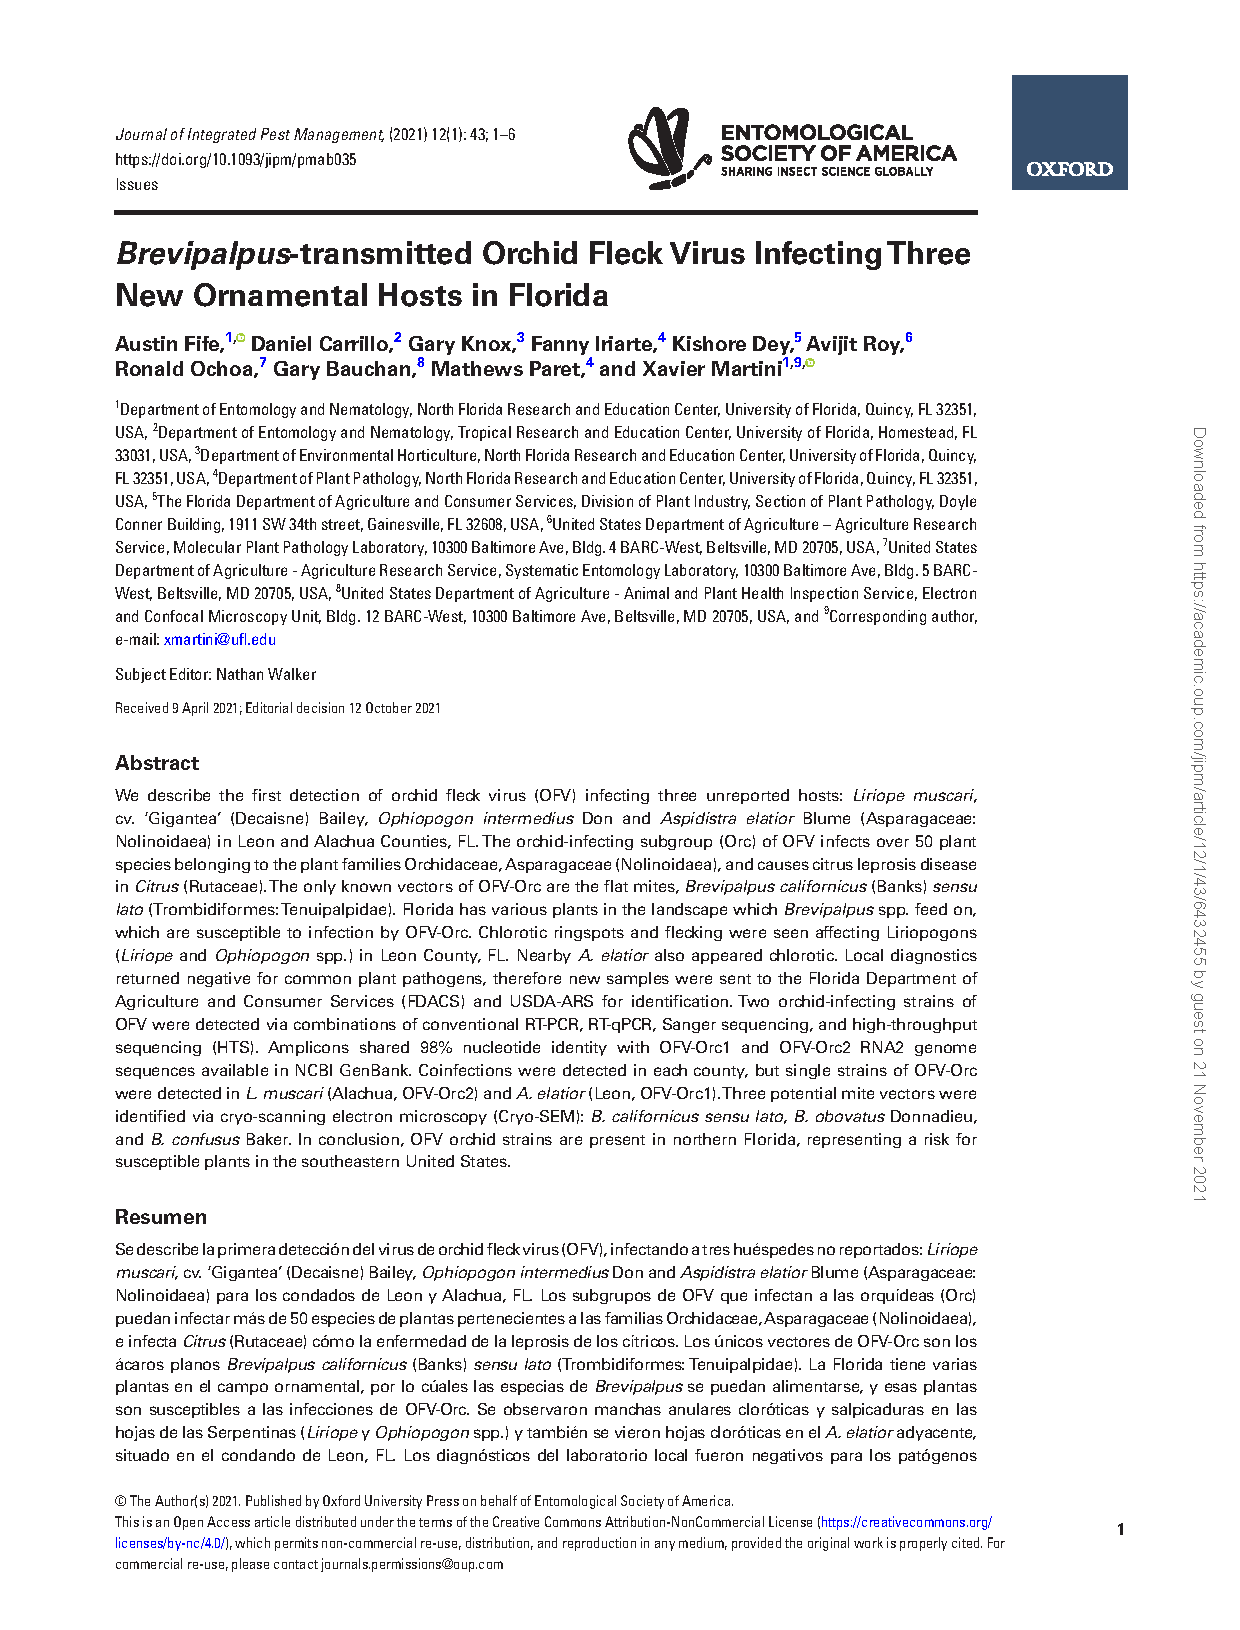
\includepdf[pages=1,pagecommand=\stepcounter{appendixVal}\stepcounter{appendixVal}\chapter {\textit{Brevipalpus}-TRANSMITTED ORCHID FLECK VIRUS INFECTING THREE NEW ORNAMENTAL HOSTS IN FLORIDA}, scale=0.93, offset=0.75 -1cm]{pubs/ofv_brevi_report.pdf}

\setlength{\footskip}{3.2em}

\includepdf[pages={2-last}, pagecommand={\thispagestyle{plain}}, fitpaper = true]{pubs/ofv_brevi_report.pdf}

\let\chapter\appendixChapter

\titleformat{\chapter }[hang]{\uppercase}{}{0pt}{\centering\realSingleSpace\ifdocBody CHAPTER \Alph{appendixVal}\\[-5pt] \fi}\raggedright\doublespacing

\docBodyfalse
\setcounter{secnumdepth}{-1}

\realSingleSpace

\hypertarget{references}{%
\chapter*{REFERENCES}\label{references}}
\addcontentsline{toc}{chapter}{REFERENCES}

\hypertarget{refs}{}
\begin{CSLReferences}{1}{1}
\leavevmode\vadjust pre{\hypertarget{ref-Baker1987}{}}%
\textbf{Baker, E. W., and D. M. Tuttle}. \textbf{1987}. The false spider mites of {Mexico} ({Tenuipalpidae}: {Acari}). (technical report No. 1706). The {United States} Department of Agriculture - Agricultural Research Service.

\leavevmode\vadjust pre{\hypertarget{ref-Bates2015}{}}%
\textbf{Bates, D., M. Mächler, B. Bolker, and S. Walker}. \textbf{2015}. Fitting linear mixed-effects models using {lme4}. Journal of Statistical Software. 67: 1--48, DOI:\href{https://doi.org/10.18637/jss.v067.i01}{10.18637/jss.v067.i01}.

\leavevmode\vadjust pre{\hypertarget{ref-Beard2015}{}}%
\textbf{Beard, J. J., R. Ochoa, W. E. Braswell, and G. R. Bauchan}. \textbf{2015}. {\emph{Brevipalpus phoenicis}} {(Geijskes)} species complex ({Acari}: {Tenuipalpidae}) \textemdash a closer look. Zootaxa. 3944: 1, DOI:\href{https://doi.org/10.11646/zootaxa.3944.1.1}{10.11646/zootaxa.3944.1.1}.

\leavevmode\vadjust pre{\hypertarget{ref-Biemond2013}{}}%
\textbf{Biemond, P. C., O. Oguntade, P. L. Kumar, T. J. Stomph, A. J. Termorshuizen, and P. C. Struik}. \textbf{2013}. Does the informal seed system threaten cowpea seed health? Crop Protection. 43: 166--174, DOI:\href{https://doi.org/10.1016/j.cropro.2012.09.007}{10.1016/j.cropro.2012.09.007}.

\leavevmode\vadjust pre{\hypertarget{ref-Bischl2016}{}}%
\textbf{Bischl, B., M. Lang, L. Kotthoff, J. Schiffner, J. Richter, E. Studerus, G. Casalicchio, and Z. M. Jones}. \textbf{2016}. \href{https://jmlr.org/papers/v17/15-066.html}{{mlr}: Machine learning in {R}}. Journal of Machine Learning Research. 17: 1--5.

\leavevmode\vadjust pre{\hypertarget{ref-Broussard2007}{}}%
\textbf{Broussard, M. C.} \textbf{2007}. A horticultural study of {\emph{Liriope}} and {\emph{Ophiopogon}}: Nomenclature, morphology, and culture (PhD thesis). Louisiana State University, Department of Horticulture.

\leavevmode\vadjust pre{\hypertarget{ref-vanBuuren2011}{}}%
\textbf{Buuren, S. van, and K. Groothuis-Oudshoorn}. \textbf{2011}. \href{https://www.jstatsoft.org/v45/i03/}{{mice}: {Multivariate} {Imputation} by {Chained} {Equations} in {R}}. Journal of Statistical Software. 45: 1--67.

\leavevmode\vadjust pre{\hypertarget{ref-Card2018}{}}%
\textbf{Card, D. C., B. W. Perry, R. H. Adams, D. R. Schield, A. S. Young, A. L. Andrew, T. Jezkova, G. I. M. Pasquesi, N. R. Hales, M. R. Walsh, M. R. Rochford, F. J. Mazzotti, K. M. Hart, M. E. Hunter, and T. A. Castoe}. \textbf{2018}. Novel ecological and climatic conditions drive rapid adaptation in invasive {Florida} {Burmese} pythons. 27: 4744--4757, DOI:\href{https://doi.org/10.1111/mec.14885}{10.1111/mec.14885}.

\leavevmode\vadjust pre{\hypertarget{ref-Chang2019}{}}%
\textbf{Chang, W.} \textbf{2019}. \href{https://CRAN.R-project.org/package=webshot}{{webshot:} Take screenshots of web pages}.

\leavevmode\vadjust pre{\hypertarget{ref-Chapman2017}{}}%
\textbf{Chapman, D., B. V. Purse, H. E. Roy, and J. M. Bullock}. \textbf{2017}. Global trade networks determine the distribution of invasive non-native species. Global Ecology and Biogeography. 26: 907--917, DOI:\href{https://doi.org/10.1111/geb.12599}{10.1111/geb.12599}.

\leavevmode\vadjust pre{\hypertarget{ref-Coomes2015}{}}%
\textbf{Coomes, O. T., S. J. McGuire, E. Garine, S. Caillon, D. McKey, E. Demeulenaere, D. Jarvis, G. Aistara, A. Barnaud, P. Clouvel, L. Emperaire, S. Louafi, P. Martin, F. Massol, M. Pautasso, C. Violon, and J. Wencélius}. \textbf{2015}. Farmer seed networks make a limited contribution to agriculture? Four common misconceptions. Food Policy. 56: 41--50, DOI:\href{https://doi.org/10.1016/j.foodpol.2015.07.008}{10.1016/j.foodpol.2015.07.008}.

\leavevmode\vadjust pre{\hypertarget{ref-Eddelbuettel2018}{}}%
\textbf{Eddelbuettel, D., and J. J. Balamuta}. \textbf{2018}. {Extending \emph{R} with \emph{C++}: A Brief Introduction to \emph{Rcpp}}. The American Statistician. 72: 28--36, DOI:\href{https://doi.org/10.1080/00031305.2017.1375990}{10.1080/00031305.2017.1375990}.

\leavevmode\vadjust pre{\hypertarget{ref-Fantz2008b}{}}%
\textbf{Fantz, P. R.} \textbf{2008}. Species of {\emph{Liriope}} cultivated in the southeastern {United States}. {HortTechnology}. 18: 343--348, DOI:\href{https://doi.org/10.21273/horttech.18.3.343}{10.21273/horttech.18.3.343}.

\leavevmode\vadjust pre{\hypertarget{ref-Fantz2009}{}}%
\textbf{Fantz, P. R.} \textbf{2009}. Names and species of {\emph{Ophiopogon}} cultivated in the southeastern {United States}. {HortTechnology}. 19: 385--394, DOI:\href{https://doi.org/10.21273/hortsci.19.2.385}{10.21273/hortsci.19.2.385}.

\leavevmode\vadjust pre{\hypertarget{ref-Fantz2015}{}}%
\textbf{Fantz, P. R., D. Carey, T. Avent, and J. Lattier}. \textbf{2015}. Inventory, descriptions, and keys to segregation and identification of liriopogons cultivated in the southeastern {United States}. {HortScience}. 50: 957--993, DOI:\href{https://doi.org/10.21273/hortsci.50.7.957}{10.21273/hortsci.50.7.957}.

\leavevmode\vadjust pre{\hypertarget{ref-Feinerer2008}{}}%
\textbf{Feinerer, I., K. Hornik, and D. Meyer}. \textbf{2008}. \href{https://www.jstatsoft.org/v25/i05/}{Text mining infrastructure in {R}}. Journal of Statistical Software. 25: 1--54.

\leavevmode\vadjust pre{\hypertarget{ref-Fox2019}{}}%
\textbf{Fox, J., and S. Weisberg}. \textbf{2019}. \href{https://socialsciences.mcmaster.ca/jfox/Books/Companion/}{An {R} companion to applied regression}, Third. ed. Sage, Thousand Oaks {CA}.

\leavevmode\vadjust pre{\hypertarget{ref-Gordon1998}{}}%
\textbf{Gordon, D. R.} \textbf{1998}. Effects of invasive, non-indigenous plant species on ecosystem processes: Lessons from {Florida}. Ecological Applications. 8: 975--989, DOI:\href{https://doi.org/10.1890/1051-0761(1998)008\%5B0975:eoinip\%5D2.0.co;2}{10.1890/1051-0761(1998)008{[}0975:eoinip{]}2.0.co;2}.

\leavevmode\vadjust pre{\hypertarget{ref-Grolemund2011}{}}%
\textbf{Grolemund, G., and H. Wickham}. \textbf{2011}. \href{https://www.jstatsoft.org/v40/i03/}{Dates and times made easy with {lubridate}}. Journal of Statistical Software. 40: 1--25.

\leavevmode\vadjust pre{\hypertarget{ref-Henry2021}{}}%
\textbf{Henry, L., and H. Wickham}. \textbf{2021}. \href{https://CRAN.R-project.org/package=tidyselect}{{tidyselect:} Select from a set of strings}.

\leavevmode\vadjust pre{\hypertarget{ref-Hiatt2019}{}}%
\textbf{Hiatt, D., K. Serbesoff-King, D. Lieurance, D. R. Gordon, and S. L. Flory}. \textbf{2019}. Allocation of invasive plant management expenditures for conservation: Lessons from {Florida}, {USA}. 1, DOI:\href{https://doi.org/10.1111/csp2.51}{10.1111/csp2.51}.

\leavevmode\vadjust pre{\hypertarget{ref-Hothorn2008}{}}%
\textbf{Hothorn, T., F. Bretz, and P. Westfall}. \textbf{2008}. Simultaneous inference in general parametric models. Biometrical Journal. 50: 346--363.

\leavevmode\vadjust pre{\hypertarget{ref-Hulme2008}{}}%
\textbf{Hulme, P. E., S. Bacher, M. Kenis, S. Klotz, I. Kühn, D. Minchin, W. Nentwig, S. Olenin, V. Panov, J. Pergl, P. Pyšek, A. Roques, D. Sol, W. Solarz, and M. Vilà}. \textbf{2008}. Grasping at the routes of biological invasions: A framework for integrating pathways into policy. Journal of Applied Ecology. 45: 403--414, DOI:\href{https://doi.org/10.1111/j.1365-2664.2007.01442.x}{10.1111/j.1365-2664.2007.01442.x}.

\leavevmode\vadjust pre{\hypertarget{ref-Jackman2020}{}}%
\textbf{Jackman, S.} \textbf{2020}. \href{https://github.com/atahk/pscl/}{{pscl}: Classes and methods for {R} developed in the political science computational laboratory}. United States Studies Centre, University of Sydney, Sydney, New South Wales, Australia.

\leavevmode\vadjust pre{\hypertarget{ref-Jeger2007}{}}%
\textbf{Jeger, M. J., M. Pautasso, O. Holdenrieder, and M. W. Shaw}. \textbf{2007}. Modelling disease spread and control in networks: Implications for plant sciences. New Phytologist. 174: 279--297, DOI:\href{https://doi.org/10.1111/j.1469-8137.2007.02028.x}{10.1111/j.1469-8137.2007.02028.x}.

\leavevmode\vadjust pre{\hypertarget{ref-Lenth2021}{}}%
\textbf{Lenth, R. V.} \textbf{2021}. \href{https://CRAN.R-project.org/package=emmeans}{{emmeans}: Estimated marginal means, aka least-squares means}.

\leavevmode\vadjust pre{\hypertarget{ref-Liebhold2012}{}}%
\textbf{Liebhold, A. M., E. G. Brockerhoff, L. J. Garrett, J. L. Parke, and K. O. Britton}. \textbf{2012}. Live plant imports: The major pathway for forest insect and pathogen invasions of the {US}. Frontiers in Ecology and the Environment. 10: 135--143, DOI:\href{https://doi.org/10.1890/110198}{10.1890/110198}.

\leavevmode\vadjust pre{\hypertarget{ref-Masiero2020}{}}%
\textbf{Masiero, E., D. Banik, J. Abson, P. Greene, A. Slater, and T. Sgamma}. \textbf{2020}. Molecular verification of the {UK} national collection of cultivated {\emph{Liriope}} and {\emph{Ophiopogon}} plants. Plants. 9: 558, DOI:\href{https://doi.org/10.3390/plants9050558}{10.3390/plants9050558}.

\leavevmode\vadjust pre{\hypertarget{ref-MoslonkaLefebvre2011}{}}%
\textbf{Moslonka-Lefebvre, M., A. Finley, I. Dorigatti, K. Dehnen-Schmutz, T. Harwood, M. J. Jeger, X. Xu, O. Holdenrieder, and M. Pautasso}. \textbf{2011}. Networks in plant epidemiology: From genes to landscapes, countries, and continents. Phytopathology{\textregistered}. 101: 392--403, DOI:\href{https://doi.org/10.1094/phyto-07-10-0192}{10.1094/phyto-07-10-0192}.

\leavevmode\vadjust pre{\hypertarget{ref-Mueller2021}{}}%
\textbf{Müller, K., and H. Wickham}. \textbf{2021}. \href{https://CRAN.R-project.org/package=tibble}{{tibble}: Simple data frames}.

\leavevmode\vadjust pre{\hypertarget{ref-Nelson2015}{}}%
\textbf{Nelson, M. F., and C. E. Bone}. \textbf{2015}. Effectiveness of dynamic quarantines against pathogen spread in models of the horticultural trade network. Ecological Complexity. 24: 14--28, DOI:\href{https://doi.org/10.1016/j.ecocom.2015.07.002}{10.1016/j.ecocom.2015.07.002}.

\leavevmode\vadjust pre{\hypertarget{ref-Neuwirth2014}{}}%
\textbf{Neuwirth, E.} \textbf{2014}. \href{https://CRAN.R-project.org/package=RColorBrewer}{{RColorBrewer}: Colorbrewer palettes}.

\leavevmode\vadjust pre{\hypertarget{ref-Ottolinger2019}{}}%
\textbf{Ottolinger, P.} \textbf{2019}. \href{https://CRAN.R-project.org/package=bib2df}{{bib2df}: Parse a {BibTeX} file to a data frame}.

\leavevmode\vadjust pre{\hypertarget{ref-Pautasso2014}{}}%
\textbf{Pautasso, M., and M. J. Jeger}. \textbf{2014}. Network epidemiology and plant trade networks. {AoB} {PLANTS}. 6, DOI:\href{https://doi.org/10.1093/aobpla/plu007}{10.1093/aobpla/plu007}.

\leavevmode\vadjust pre{\hypertarget{ref-Schloerke2021}{}}%
\textbf{Schloerke, B., D. Cook, J. Larmarange, F. Briatte, M. Marbach, E. Thoen, A. Elberg, and J. Crowley}. \textbf{2021}. \href{https://CRAN.R-project.org/package=GGally}{{GGally}: Extension to 'ggplot2'}.

\leavevmode\vadjust pre{\hypertarget{ref-Schoebel2014}{}}%
\textbf{Schoebel, C. N., J. Stewart, N. J. Grünwald, D. Rigling, and S. Prospero}. \textbf{2014a}. Population history and pathways of spread of the plant pathogen {\emph{Phytophthora plurivora}}. {PLoS} {ONE}. 9: e85368, DOI:\href{https://doi.org/10.1371/journal.pone.0085368}{10.1371/journal.pone.0085368}.

\leavevmode\vadjust pre{\hypertarget{ref-Schoebel2014a}{}}%
\textbf{Schoebel, C. N., J. Stewart, N. J. Grünwald, D. Rigling, and S. Prospero}. \textbf{2014b}. Correction: Population history and pathways of spread of the plant pathogen {\emph{Phytophthora plurivora}}. {PLoS} {ONE}. 9: e106209, DOI:\href{https://doi.org/10.1371/journal.pone.0106209}{10.1371/journal.pone.0106209}.

\leavevmode\vadjust pre{\hypertarget{ref-Schoebel2014b}{}}%
\textbf{Schoebel, C. N., J. Stewart, N. J. Grünwald, D. Rigling, and S. Prospero}. \textbf{2014c}. Correction: Population history and pathways of spread of the plant pathogen {\emph{Phytophthora plurivora}}. {PLoS} {ONE}. 9: e105259, DOI:\href{https://doi.org/10.1371/journal.pone.0105259}{10.1371/journal.pone.0105259}.

\leavevmode\vadjust pre{\hypertarget{ref-Simberloff1997}{}}%
\textbf{(Strangers in paradise ) }. \textbf{1997}. Strangers in paradise. Island Press, Washington, D.C.

\leavevmode\vadjust pre{\hypertarget{ref-Tennekes2018}{}}%
\textbf{Tennekes, M.} \textbf{2018}. {tmap}: Thematic maps in {R}. Journal of Statistical Software. 84: 1--39, DOI:\href{https://doi.org/10.18637/jss.v084.i06}{10.18637/jss.v084.i06}.

\leavevmode\vadjust pre{\hypertarget{ref-Tierney2021}{}}%
\textbf{Tierney, N., D. Cook, M. McBain, and C. Fay}. \textbf{2021}. \href{https://CRAN.R-project.org/package=naniar}{Naniar: Data structures, summaries, and visualisations for missing data}.

\leavevmode\vadjust pre{\hypertarget{ref-Wallace2016}{}}%
\textbf{Wallace, R. D., C. T. Bargeron, D. J. Moorhead, and J. H. LaForest}. \textbf{2016}. {IveGot}1: Reporting and tracking invasive species in {Florida}. 15: 51--62, DOI:\href{https://doi.org/10.1656/058.015.sp805}{10.1656/058.015.sp805}.

\leavevmode\vadjust pre{\hypertarget{ref-Wang2014}{}}%
\textbf{Wang, G.-Y., Y. Meng, J.-L. Huang, and Y.-P. Yang}. \textbf{2014}. Molecular phylogeny of {\emph{Ophiopogon}} {({Asparagaceae})} inferred from nuclear and plastid {DNA} sequences. Systematic Botany. 39: 776--784, DOI:\href{https://doi.org/10.1600/036364414x682201}{10.1600/036364414x682201}.

\leavevmode\vadjust pre{\hypertarget{ref-Westphal2007}{}}%
\textbf{Westphal, M. I., M. Browne, K. MacKinnon, and I. Noble}. \textbf{2007}. The link between international trade and the global distribution of invasive alien species. Biological Invasions. 10: 391--398, DOI:\href{https://doi.org/10.1007/s10530-007-9138-5}{10.1007/s10530-007-9138-5}.

\leavevmode\vadjust pre{\hypertarget{ref-Wickham2019b}{}}%
\textbf{Wickham, H.} \textbf{2019}. \href{https://CRAN.R-project.org/package=stringr}{{stringr}: Simple, consistent wrappers for common string operations}.

\leavevmode\vadjust pre{\hypertarget{ref-Wickham2021b}{}}%
\textbf{Wickham, H., J. Hester, and W. Chang}. \textbf{2021}. \href{https://CRAN.R-project.org/package=devtools}{{devtools}: Tools to make developing {R} packages easier}.

\leavevmode\vadjust pre{\hypertarget{ref-Williams2007}{}}%
\textbf{Williams, D. A., E. Muchugu, W. A. Overholt, and J. P. Cuda}. \textbf{2007}. Colonization patterns of the invasive {Brazilian} peppertree, {\emph{Schinus terebinthifolius}}, in {Florida}. 98: 284--293, DOI:\href{https://doi.org/10.1038/sj.hdy.6800936}{10.1038/sj.hdy.6800936}.

\leavevmode\vadjust pre{\hypertarget{ref-Zeileis2008}{}}%
\textbf{Zeileis, A., C. Kleiber, and S. Jackman}. \textbf{2008}. \href{http://www.jstatsoft.org/v27/i08/}{Regression models for count data in {R}}. Journal of Statistical Software. 27.

\end{CSLReferences}
\hypertarget{biographical-sketch}{%
\chapter*{BIOGRAPHICAL SKETCH}\label{biographical-sketch}}
\addcontentsline{toc}{chapter}{BIOGRAPHICAL SKETCH}

Austin N Fife received his B.S. degree in biology - zoology emphasis at Brigham Young University - Idaho at Rexburg. During his undergraduate degree, he conducted research on the distribution of the endemic St.~Anthony Dunes Tiger Beetle \emph{Cicendela arenicola}. He went on to receive a M.S. in entomology at the University of Idaho while working at the Kimberly Research and Extension Center on potato psyllids \emph{Bactericera cockerelli} and host plant resistance. He received his PhD in entomology and nematology at the University of Florida in 2021 while working at the North Florida Research and Education Center in Quincy, FL. There, his research focused on \emph{Phyllocoptes fructiphilus} and \emph{Rose rosette emaravirus}, the causal agent of Rose Rosette Disease. His research covered a variety of topics, including acarology, chemical ecology, induced plant defenses, biological control, and plant-pathogen-arthropod interactions. As a former Eagle Scout from Idaho, he loves to spend time outdoors with his wife, Liz and his two (soon to be three) lovely daughters, Violet, Juniper and \{insert plant name here\}.}                       % This imports the body chapters included in the _bookdown.yml file,
% you can add as many chapters as you need

%%%%%%%%%%%%%%%%%%%%%%%%%%%%%%%%%
% APPENDICES                    %
%%%%%%%%%%%%%%%%%%%%%%%%%%%%%%%%%

% If you have multiple appendices, add them as new chapters in the 98--appendix.Rmd file


%%%%%%%%%%%%%%%%%%%%%%%%%%%%%%%%%
% LIST OF REFERENCES            %
%%%%%%%%%%%%%%%%%%%%%%%%%%%%%%%%%

% provided by file 98-references.Rmd

%%%%%%%%%%%%%%%%%%%%%%%%%%%%%%%%%
% BIOGRAPHICAL SKETCH
%%%%%%%%%%%%%%%%%%%%%%%%%%%%%%%%%

% provided by file 99--biography.Rmd


\end{document}
